\documentclass[conference]{IEEEtran}
% If the IEEEtran.cls has not been installed into the LaTeX system files,
% manually specify the path to it.  e.g.
% \documentclass[conference]{./IEEEtran}

% Add and required packages here
\usepackage{graphicx,times,amsmath}

% To handle Icelandic letters
\usepackage[utf8]{inputenc}
\usepackage[T1]{fontenc}


%\usepackage{subcaption}
%
%% Training subcaption package to comply with
%% IEEE standards. We can ignore the warning
%% generated by caption.sty which is due to 
%% the redefinition of \@makecaption
%\DeclareCaptionLabelSeparator{periodspace}{.\quad}
%\captionsetup{font=footnotesize,labelsep=periodspace,singlelinecheck=false}
%\captionsetup[sub]{font=footnotesize,singlelinecheck=true}


% Correct bad hyphenation here
\hyphenation{op-tical net-works semi-conduc-tor IEEEtran}

% To create the author's affliation portion using \thanks
\IEEEoverridecommandlockouts

\textwidth 178mm
\textheight 239mm
\oddsidemargin -7mm
\evensidemargin -7mm
\topmargin -6mm
\columnsep 5mm

\begin{document}

% Project title: keep the \ \\ \LARGE\bf in it to leave enough margin.
\title{\ \\ \LARGE\bf Modern AI for Games - Report on Individual Assignment}

\author{Björn Þór Jónsson - \texttt{bjrr@itu.dk}}

% Uncomment out the following line for invited papers
%\specialpapernotice{(Invited Paper)}

% Make the title area
\maketitle

\begin{abstract}
Following is a report on using AI methods to\textbf{} control an agent in the game of Ms PacMan.  The discussed methods are:  Genetic Algorithm with a Behaviour Tree; Artificial Neural Network with Backpropagation; and Monte Carlo Tree Search.
\end{abstract}

\section{Introduction}
\PARstart{T}{his} report outlines the implementation and results gained from the use of Artificial Intelligence methods to control Ms PacMan in a provided test bed framework \cite{msPacManFramework}.  The three methods chosen to implement are based on an Evolutionary Algorithm, a Neural Network with Backpropagation, and Monte Carlo Tree Search.

The following sections describe each implementation.  The methods were implemented in Java and the sections will contain references to the Java package names containing the relevant implementation classes.

Plots of the generated data - performance measures an experiments - were made with simple R scripts that can be found in the \texttt{plots} directory within the supplied implementation project.


\section{Genetic Algorithm with a Behaviour Tree}

\subsection{Behaviour Tree with prioritized tactics}

A Behaviour Tree framework was implemented - \texttt{bjrr.pacman.behaviourtree.ai.*} - and a tree constructed with a root priority selector for three tactics, based on the strategies in the \texttt{StarterPacMan} procedural controller supplied with the Ms Pac-Man vs Ghosts League framework.  The strategies are, in order of priority:  
\begin{itemize}
	\item Get away from any non-edible ghost that is in close proximity
	\item Go after the nearest edible ghost
	\item Go to the nearest pill/power pill
\end{itemize}
A controller constructing this tree can be seen in \texttt{bjrr.pacman.behaviourtree\\.BehaviourTreePacManController} and an initial sketch of the tree layout can be seen in figure~\ref{behaviourTreeSketch}.

\begin{figure}[htp]
\centerline{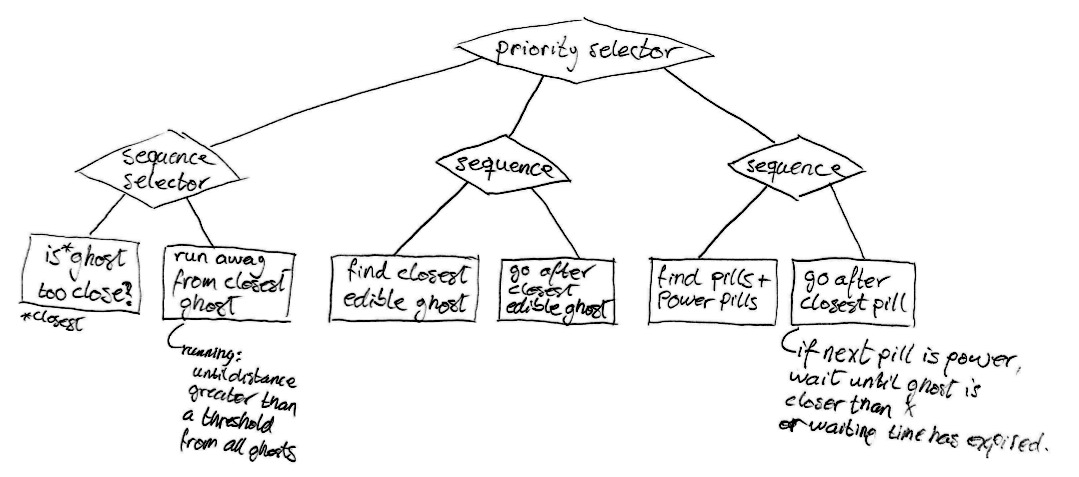
\includegraphics[width=1\columnwidth]{BehaviourTreeSketch.png}}
\caption{Sketch of a Behaviour Tree prioritizing the control of Ms PacMan}
\label{behaviourTreeSketch}
\end{figure}

\subsection{Genetic Evolution of tactical attribute values}

Within the tasks of this constructed behaviour tree are three attributes governing tactical decisions by the Ms PacMan agent.  Those attributes are stored in a centralized memory - a black board class \texttt{bjrr.pacman.behaviourtree.PacManBlackboard} - accessible by all tasks of the tree.  The attributes are used in the tasks \texttt{IsGhostTooClose} and \texttt{GoAfterClosestAvailablePill} and are:
\begin{itemize}
	\item \texttt{MIN\_GHOST\_DISTANCE} in \texttt{IsGhostTooClose} to determine when to run away from a non-edible ghost.
	\item \texttt{MAX\_POWER\_PILL\_DISTANCE} in \texttt{GoAfterClosestAvailablePill} used to define how close to a power pill Ms PacMan can get, before she turns away from it.
	\item \texttt{POWER\_PILL\_WALK\_AWAY\_DISTANCE} also in \texttt{GoAfterClosestAvailablePill} declaring for how long Ms PacMan maintains her chosen course away from a power pill.
\end{itemize}

The combined use of those attributes results in the tactic where Ms PacMan never eats a power pill free-willingly, but may run away from ghosts towards a power pill, luring them to close proximity when she eats one.  By using this tactic there will initially be a short distance to edible ghosts after eating a power pill.

A Genetic Algorithm was used to obtain optimal values for those attributes - \texttt{bjrr.pacman.ga.PacManGeneticAlgorithm} - evolving them in successive generations of genes - \texttt{bjrr.pacman.ga.PacManGeneForBehaviourTree}.

It was chosen to work with a population of size 500.  The Genetic Algorithm's fitness function consists of the score results from one run of a Ms PacMan controller without visuals - \texttt{bjrr.pacman.ga\\.GeneticAlgorithmPacManController}.  That controller constructs a Behaviour Tree and populates its central memory with attribute values from the gene being evaluated for fitness.

Several options were considered for the reproduction of the next generation.  From the example applications discussed in section 2.4 of~\cite{eiben2003introduction} the Evolutionary Algorithm in section 2.4.1 (The 8-Queens Problem) was chosen as a model, where the best 2 of random 5 individuals / genes from the current population are chosen to be parents, and their children replace the two worst individuals in the population.

Offspring reproduction from the two chosen parents is done by giving each child an attribute value from either parent with equal chance.  The gene of each child is then mutated by giving each attribute a new random value with a predefined probability.  The random values are chosen within an upper bound of 100, as most values in the files in data/distance directory of the Ms PacMan framework were observed to be lower than 100.  Mutation probabilities of .125 and .05 were tried and the evolution with each can be seen in figure~\ref{geneticEvolution}.

\subsection{Performance}

While running the Genetic Algorithm, evolution was set to continue while the difference between the best and worst fitness, within the current generation, was over the score threshold of 100, and while the all time best fitness from all generations and that of this generation was above the same threshold.  This goal was not reached after several thousands of generations and the evolution was arbitrarily stopped when the fitness values were observed to be similar between generations.

When the Genetic Algorithm had produced two thousand generations, the best fitness obtained from each generation fluctuated in the range of Ms PacMan scores between 7000 and 8000, as can be seen in figure~\ref{geneticEvolution}.


% image arrangement based on http://tex.stackexchange.com/a/133058/64219
\begin{figure}
\centering
\raisebox{-.5\height}{%
  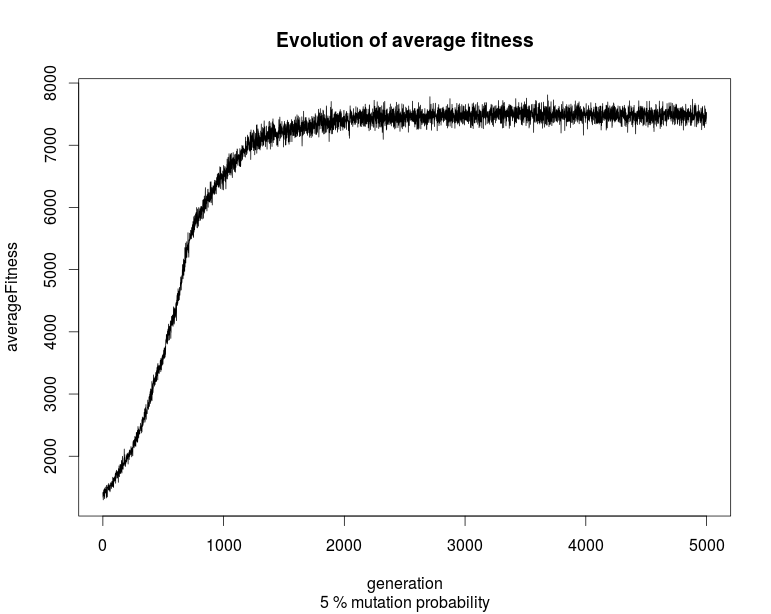
\includegraphics[width=\columnwidth]{evolutionOfAverageFitness_5_percent_mutation_probability.png}%
}\qquad
\raisebox{-.5\height}{%
  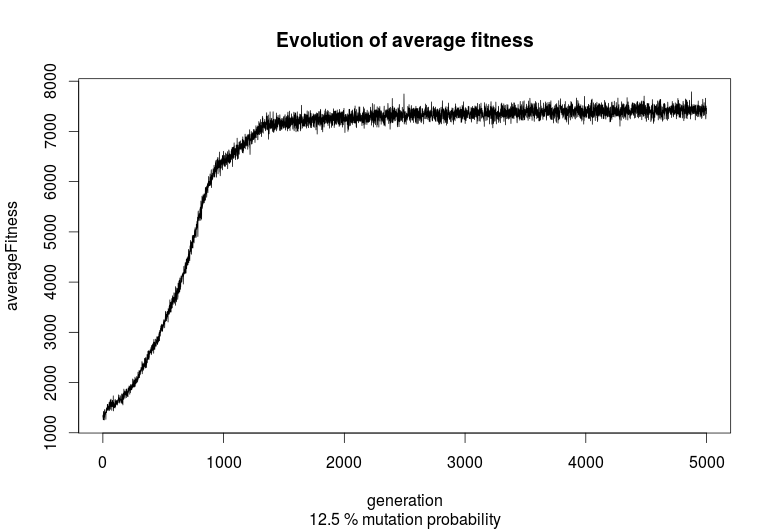
\includegraphics[width=\columnwidth]{evolutionOfAverageFitness_12dot5_percent_mutation_probability.png}%
}
\caption{Evolution of fitness through generations of attribute value genes for a Ms PacMan controller.  Each plot is from an evolution with different probabilities of mutation, 5\% and 12.5\%, and apparently the mutation probabilities do not change much in the progress of the evolution.}
\label{geneticEvolution}
\end{figure}



\section{Neural Network with Backpropagation}

\subsection{Inputs}

In an attempt to explore the benefits of providing different kinds of inputs for training a Neural Network with Backpropagation, new attributes were added to the DataTuple class that was provided in a data recording lab code package - \texttt{bjrr.pacman.ann.dataRecording.DataTuple}.  Those new attributes are the booleans: \texttt{lastDirectionSame}, indicating whether PacMan is about to choose the same move as he did on the previous game tick; \texttt{isClosestGhostMovingInSameDirectionAsPacman}, \texttt{isClosestGhostEdible}; and the integers:  \texttt{distanceToClosestPill}, \texttt{distanceToClosestPowerPill}, and \texttt{distanceToClosestGhost}.  The attributes are normalized with the normalization methods provided in the DataTuple class.  A sketch of those inputs can be seen in figure~\ref{annSketch}.

Two input sets were tried for training the Neural Network.  The first input set contains only values collected in the original version of the data collection package.  The second input set contains the new attributes, outlined above, in a mix with some of the previously provided attributes.

Input set 1 consists of:  
\begin{itemize}
	\item Ms PacMan current level
	\item Ms PacMan position
	\item Number of pills left
	\item Number of Power pills left
	\item Whether each of the ghosts is edible
	\item Distances to each of the ghosts
\end{itemize}

Input set 2 consists of:
\begin{itemize}
	\item Ms PacMan current level
	\item Ms PacMan position
	\item Number of pills left
	\item Number of Power pills left
	\item Whether Ms PacMan last direction is same as the chosen one
	\item Distance to closest pill
	\item Distance to closest power pill
	\item Distance to closest ghost
	\item Whether the closest ghost is edible
	\item Whether the closest ghost is moving in the same direction as Ms PacMan
\end{itemize}


\subsection{Training}
The two input sets were tried for training the Neural Network, and for each of them, two different numbers of hidden neurons were tried.  For each of those four combinations, two different learning rate configurations were tried, accounting for a total of eight training sessions.  Each training session lasted for more than five hundred thousand iterations / epochs and in figure~\ref{annTrainingEpochs} plots are shown of training epochs up to 550.000 against the rate of error in the output prediction of the network.

For training, a two-layer neural network was constructed (as defined in \cite{Han:2005:DMC:1076797}, section 9.2.1), with one hidden layer layer.  The number of neurons for the hidden layer was chosen by considering rules of thumb presented in \cite{heaton2008introduction}, chapter 5:
\begin{itemize}
	\item The number of hidden neurons should be between the size of the input layer and the size of the output layer.
	\item The number of hidden neurons should be 2/3 the size of the input layer, plus the size of the output layer.
	\item The number of hidden neurons should be less than twice the size of the input layer.
\end{itemize}

The latter two rules of thumb were implemented for the training sessions.  

For the last rule, which states \textit{that the number hidden neurons should be less than twice the size of the input layer}, the multiplier 1.7 was used against the number of input neurons to obtain the hidden neuron count.  This resulted in a slightly larger number of neurons (20 versus 12) and in somewhat less error rate in the predictions output by the network, as can be seen in figure~\ref{annTrainingEpochs}.

Both a fixed learning rate of 0.1, and a learning rate of 1/t (where t is increased on every 100th epoch, as suggested in the labs), were tested for training the neural network.  The fixed learning rate gave a substantially better result in network prediction, as can be seen in figure~\ref{annTrainingEpochs} when comparing the plots with thin straight lines (decreasing learning rate) with the pots depicting fluctuating lines (fixed learning rate); the decreasing learning rate results in prediction errors of around and above 25\% and the fixed learning rate results in prediction errors below 20\%.

Difference in prediction performance between the two input sets is barely observable, though input set 1, which does not contain the custom attributes, performs slightly better, as can be seen when comparing the second and last plots in figure~\ref{annTrainingEpochs}.


\subsection{Performance}

The training data consisted of data recordings from five games of Ms PacMan played by the author of this report, which happens to be quite bad at playing the game.  So a controller using a neural network trained with this data could not be expected to perform well.  

The actual result of using a trained network in a Ms PacMan controller is even worse than expected, where Ms PacMan starts by choosing sensible moves, but soon gets stuck in a corner without choosing a move leading the agent onto a path out of that corner.  The reason for that behaviour has not been investigated further and so is yet unknown.

An embarrassing average score of 255 was obtained from running a Ms PacMan game simulation 100 times with one of the trained networks, and the average score could go as low as 71 for other networks.



\subsection{Implementation}
The neural network implementation - \texttt{bjrr.pacman.ann.feedforwardbackpropagation} - is straight forward with a Java class for the network, and one class each for the layers and neurons.  Connections are also defined in their own Java class, whose instances are shared between connecting neurons.  A Backpropagation class was created to perform the training iterations.  A sketch of the code structure can be seen in figure~\ref{annImplementationSketch}.

The Java class \texttt{bjrr.pacman.ann\\.FeedforwardBackpropagationPacmanTraining} was created to set up the network for training, computing the number of hidden input neurons and managing the learning rate during the training iterations.  A controller for trying out the trained networks can be found in \texttt{bjrr.pacman.ann\\.FeedforwardBackpropagationPacmancontroller}.

Before starting this straight forward implementation, I was exposed to a more sophisticated implementation when reading chapters two and five of \cite{heaton2008introduction}, which introduce the concept of using matrices to represent weights and bias for each neuron, and how matrix arithmetic can be used to update the weights during the backpropagation of errors.  In addition to specifying a learning rate, the implementation discussed in chapter five of that book uses the concept of momentum, which scales the learning from the previous iteration before applying it to the current iteration; it “specifies how much of an effect the previous training iteration will have on the current iteration”\cite{heaton2008introduction}.  It was interesting to learn about that concept, where "Acting like a lowpass filter, momentum allows the network to ignore small features in the error surface. Without momentum a network can get stuck in a shallow local minimum. With momentum a network can slide through such a minimum"\cite{traingdm}.

Supplied with the book is an implementation of a neural network and training with backpropagation (along with other methods of training) \cite{jeffheaton-bookcode} and my first inclination was to base my own implementation on that code.  Then I realized it would be hard to not just copy paste the relevant code and even more time consuming than doing my own thing from scratch.  So even though it was interesting to learn about the use of matrix arithmetic to update the network weights and biases, I decided to skip using matrices and the simple implementation discussed above.

One class I did copy straight from that book code though, and that is \texttt{SerialzieObject}, for saving and loading the trained network.


\begin{figure}[htp]
\centerline{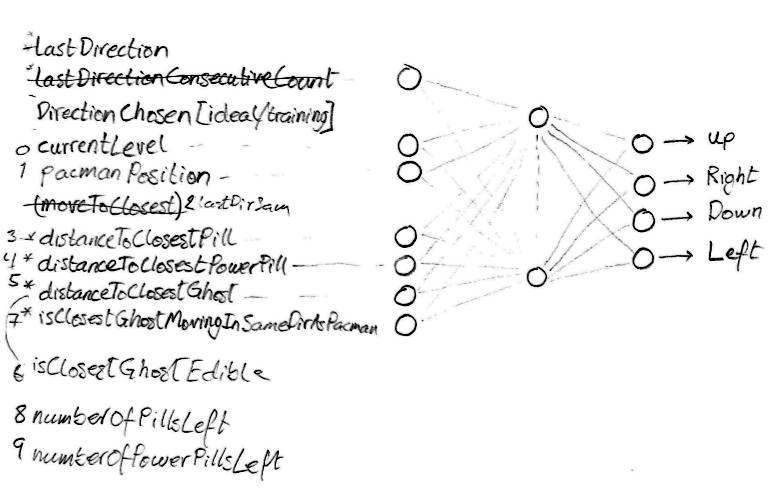
\includegraphics[width=1\columnwidth]{ANNsketch.png}}
\caption{Sketch of Neural Network inputs and outputs.}
\label{annSketch}
\end{figure}


\begin{figure}[htp]
\centerline{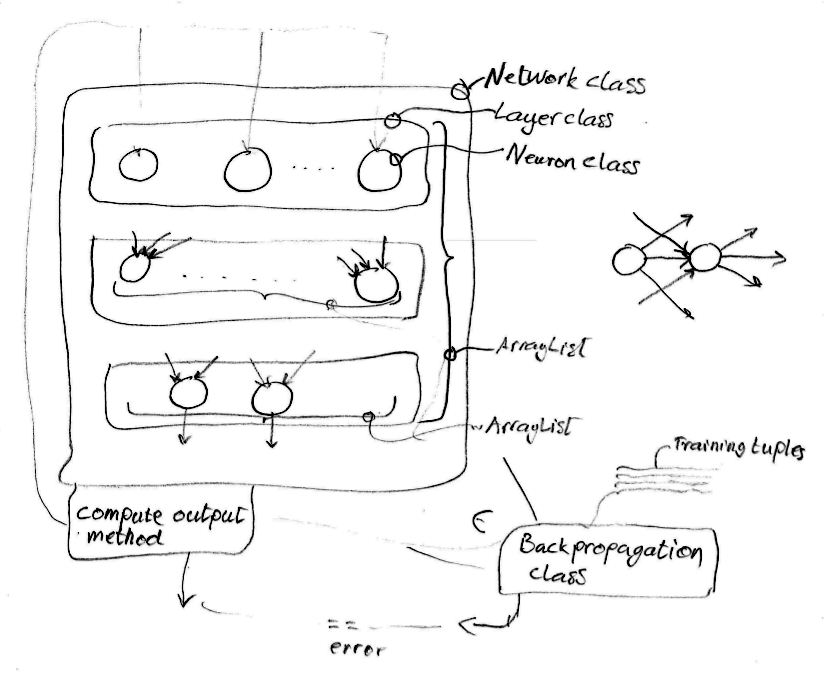
\includegraphics[width=1\columnwidth]{ANNimplementationSketch.png}}
\caption{Sketch of main components in a straightforward Artificial Neural Network implementation.}
\label{annImplementationSketch}
\end{figure}


\begin{figure}
\centering
\raisebox{-.5\height}{%
  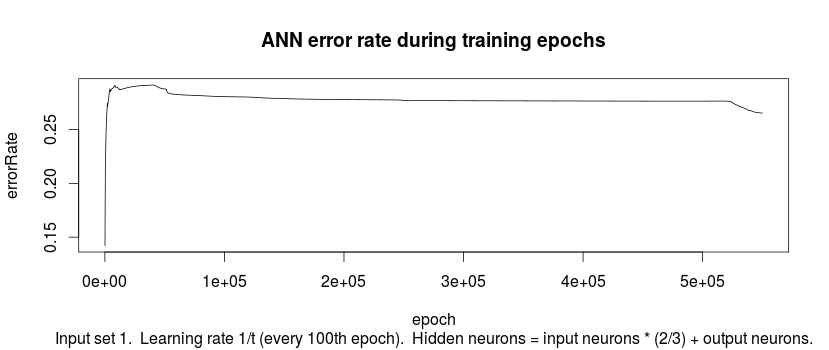
\includegraphics[width=\columnwidth]{ANNtraining__inputSet1__decreasingLearningRate__hiddenNeuronsTwoThirdsOfInput.png}%
}\qquad
\raisebox{-.5\height}{%
  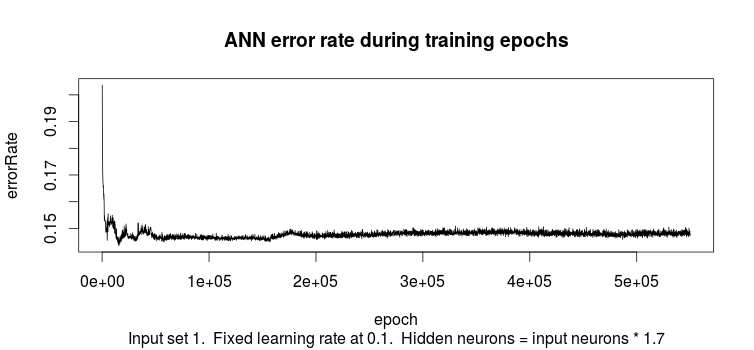
\includegraphics[width=\columnwidth]{ANNtraining__inputSet1__fixedLearningRate__hiddenNeuronsLessThanTwiceInputSet.png}%
}\qquad
\raisebox{-.5\height}{%
  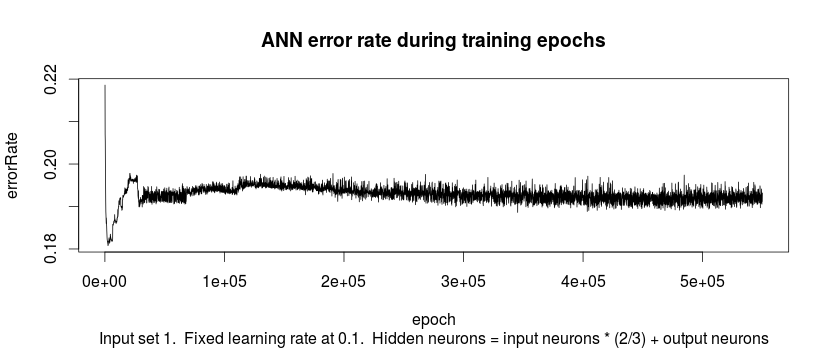
\includegraphics[width=\columnwidth]{ANNtraining__inputSet1__fixedLearningRate__hiddenNeuronsTwoThirdsOfInput.png}%
}\qquad
\raisebox{-.5\height}{%
  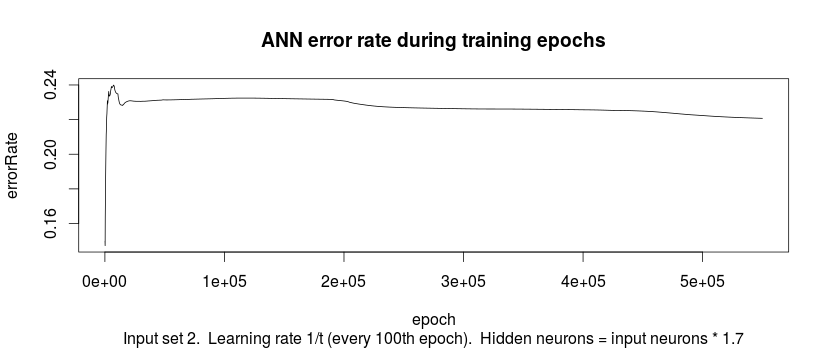
\includegraphics[width=\columnwidth]{ANNtraining__inputSet2__decreasingLearningRate__hiddenNeuronsLessThanTwiceInputSet.png}%
}\qquad
\raisebox{-.5\height}{%
  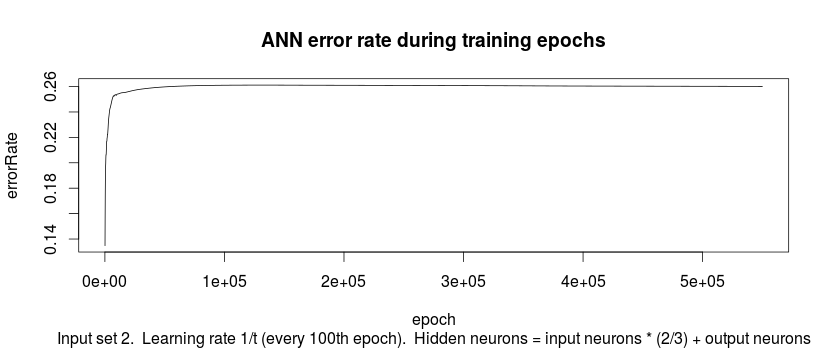
\includegraphics[width=\columnwidth]{ANNtraining__inputSet2__decreasingLearningRate__hiddenNeuronsTwoThirdsOfInput.png}%
}\qquad
\raisebox{-.5\height}{%
  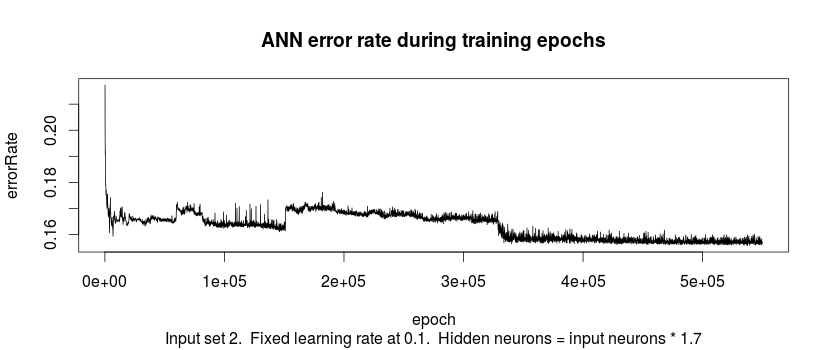
\includegraphics[width=\columnwidth]{ANNtraining__inputSet2__fixedLearningRate__hiddenNeuronsLessThanTwiceInputSet.png}%
}
\caption{Error rates, in the predictions of trained neural networks, against 550.000 training iterations.  Fixed and decreasing learning rates were tried, with the former giving better results.  A higher number of hidden neurons, chosen from two used rules of thumb, gives a slightly better result.}
\label{annTrainingEpochs}
\end{figure}



\section{Monte Carlo Tree Search}

\subsection{Implementation}

In preparation for using MCTS in a Ms PacMan controller, the partial tutorial implementation provided in the labs was completed - \texttt{bjrr.tutorial.mcts}.

The tutorial implementation was then adapted for use in a Ms PacMan controller - \texttt{bjrr.pacman.mcts}.  Specifically the methods in \texttt{bjrr.pacman.mcts.UCT} for selection (\texttt{TreePolicy}), expansion (\texttt{Expand}), playouts / simulation (\texttt{DefaultPolicy} or \texttt{GeneticBehaviourTreePolicy}) and backpropagation (\texttt{Backpropagate}) were adapted to use the Ms Pac-Man vs Ghosts League framework methods to obtain the possible moves at any given state during expansion and to retrieve the (non-normalized) score during simulation for backpropagation.

Instead of having a predefined number of iterations for building the MCTS tree, it was decided to continue iterating while the current time was within the time due provided by the Ms PacMan framework in the getMove call.  To avoid beginning a new iteration that would take longer than the remaining available time, the average time taken by previous iterations was calculated.  As each iteration proved to take less than one millisecond, that average was deemed to be insufficient for ensuring the MCTS would finish in time to return a move.  So one millisecond was simply added to the current time when determining whether the next iteration would finish in time:\\
\texttt{while( System.currentTimeMillis() + 1 < timeDue ) \{}

Using those conditions an iteration count from over 100 to little under 700 was obtained for each move request on a five year old Ubuntu desktop with \texttt{Intel(R) Core(TM)2 Quad CPU @ 2.40GHz}.  It was interesting to observe that using debug log statements, in the MCTS iteration loop, with \texttt{System.out.println} severely skewed those time calculations; no more than one iteration was achieved with a log statement there, resulting in the controller always returning NEUTRAL moves for Ms PacMan.

Instead of applying specific conditions to “determine the short- and long-term safety and reward of a selected path” as is done in the playout strategy of \cite{pepels2012enhancements}, an attempt was made to play the PacMan game until either of it’s normal end states are reached - “when either Pac-Man loses all lives, or the 16th level is cleared”\cite{pepels2012enhancements} - and instead of manually determining PacMan’s score according to the games subgoals mentioned in the \cite{pepels2012enhancements}, we’ll simply get the score at the current state from the PacMan game framework (\texttt{Game.getScore()}).  As this may not be feasible within the time frame of 40 milliseconds, for example when the playout strategy is good enough to keep PacMan alive for a long time, we’ll instead introduce a limit on the number of iterations of the playout, or simulation.

What limit on iteration count gives the best result was to be obtained by measuring the score from one game play with the \texttt{MCTSPacmanController} with a range of iteration limits, and choosing the limit that gave the highest average score.  An average of more than one play result for each limit would have been preferable, but as the MCTS controller takes a long time, even in a simulation without any visuals, where it uses all the available time for each tick / game advancement, time only allowed one game play per iteration limit.


\subsection{Performance}

Two different playout strategies (DefaultPolicy) were be tried:
\begin{itemize}
	\item A strategy where random moves of those available at any given time for PacMan will be tried.  Ghost moves will be obtained from the StarterGhosts controller.
	\item Or a strategy where the behaviour tree controller previously discussed, with genetically evolved attribute values for controlling strategic moves, will be used to obtain PacMan moves at any given time and the ghosts will be controlled as in the previous strategy.
\end{itemize}

Resulting scores from controlling Ms PacMan with a MCTS, with varying limits on the number of MCTS iterations, can be seen in figure~\ref{mctsIterationLimitTrials}.  The iteration limits shown range from 0 to 600, where 0 is interpreted as a no limit.  The plot is quite noisy, with the scores fluctuating across a wide range between different iteration limits; the curves would probably be much smoother when an average would be taken from several played games for each iteration limit, but as mentioned before, only one game is played for each limit due to time constraints.

With the playout strategy of random movements for Ms PacMan, having no limit (0) on the number of MCTS tree building iterations gives the best result, with one comparable spike between the limits of 300 and 400.  A playout strategy using the genetically evolved controller for moves, generally gives higher scores for MCTS iteration limits around 100, as can be seen on the second plot of figure~\ref{mctsIterationLimitTrials}.

\begin{figure}
\centering
\raisebox{-.5\height}{%
  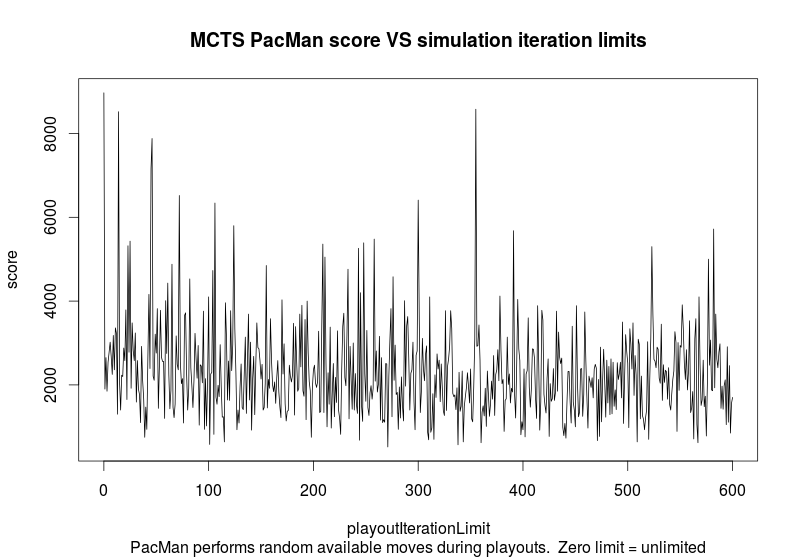
\includegraphics[width=\columnwidth]{MCTSforPacMan__DefaultPolicy__iterationLimitTrials.png}%
}\qquad
\raisebox{-.5\height}{%
  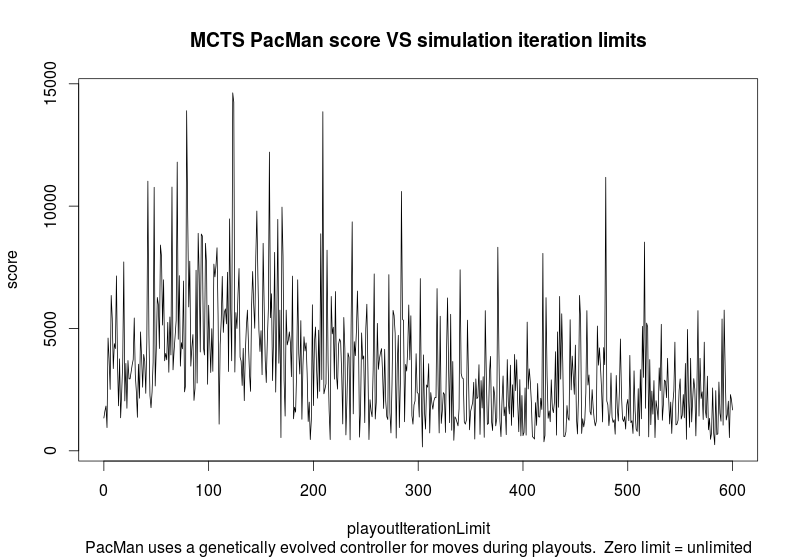
\includegraphics[width=\columnwidth]{MCTSforPacMan__GeneticControllerSimulation__iterationLimitTrials.png}%
}
\caption{Limits on MCTS iterations, used for getting moves in a Ms PacMan controller, plotted against the resulting scores.}
\label{mctsIterationLimitTrials}
\end{figure}



\section{Conclusions}
It has been interesting to try out different Artificial Intelligence techniques for controlling Ms PacMan vs the Ghosts League.  The simplest method of genetically evolving values for three strategic attributes, used in Behaviour Tree tasks, seemingly gives the consistently best results of those obtained from the implementations discussed in this report.




% Trigger a \newpage just before a given reference number in order to
% balance the columns on the last page.  Adjust the value as needed;
% it may need to be readjusted if the document is modified later.
%\IEEEtriggeratref{8}
% The "triggered" command can be changed if desired:
%\IEEEtriggercmd{\enlargethispage{-5in}}

% The references section can either be generated by hand or by an
% automatic tool like BibTeX.  If using BibTex, use the standard IEEEtran
% bibliography style.
%\bibliographystyle{IEEEtran.bst}
%
% The argument to \bibliography is/are the name(s) of your BibTeX file(s)
% that contains string definitions and bibliography database(s).
%\bibliography{IEEEabrv,SamplePaper}
%
% If you generate the bibliography by hand, or if you copy in the
% resultant .bbl file, set the second argument of \begin to the number of
% references in the bibliography (used to reserve space for the reference
% number labels box).


\bibliographystyle{IEEEtran.bst}
\bibliography{ModernAIref}


%\begin{thebibliography}{3}

%\begin{thebibliography}


%\bibitem{book}
%A.~Great, \emph{This is the book title}.\hskip 1em plus 0.5em minus 0.4em\relax
%  This is the name of the publisher, 2006.
%
%\bibitem{conf}
%F.~Author, S.~Author, and T.~NonRelatedAuthor, ``This is the paper title,'' in
%  \emph{This is the proceedings title}, 2008, pp. 1--8.
%
%\bibitem{article}
%B.~Myself, ``This is the title of the journal article,'' \emph{This is the name
%  of the journal}, pp. 1--30, 2007.
%

%\end{thebibliography}


% That's all folks...
\end{document}
